\documentclass[]{report}
\usepackage{graphicx}
\usepackage{hyperref} 
\usepackage[a4paper, lmargin=2.5cm, right=2.5cm, top=2.5cm, bottom=2.5cm]{geometry} %, headsep=1.2cm

\def\thesection{\arabic{section}}

\title{Benchmarking oneSolver with droplet instances}
\author{Bart\l{}omiej Gardas}


\begin{document}
\maketitle

\begin{abstract}
It is well established that annealing-based spin-glass solvers can ``stuck'' in local minimum, ultimately preventing 
the heuristic from reaching the ground state (\emph{i.e.}, true optimal solution). This, in fact, remains true for all heuristic 
approaches designed for optimization. Therefore, it is essential to perform testing, and benchmarking against problem
instances that are considered to be ``hard" (\emph{e.g.}, have a nontrivial structure). Herein, we investigate how well
the oneSolver performs trying to solve droplets instances encoded in two-dimensional Ising spin-glass problems. 
Similar idea has recently been incorporated to test sophisticated solvers, which are based on tensor networks, and 
and projected entangled pair states.
\end{abstract}

\begin{figure}[h!]
	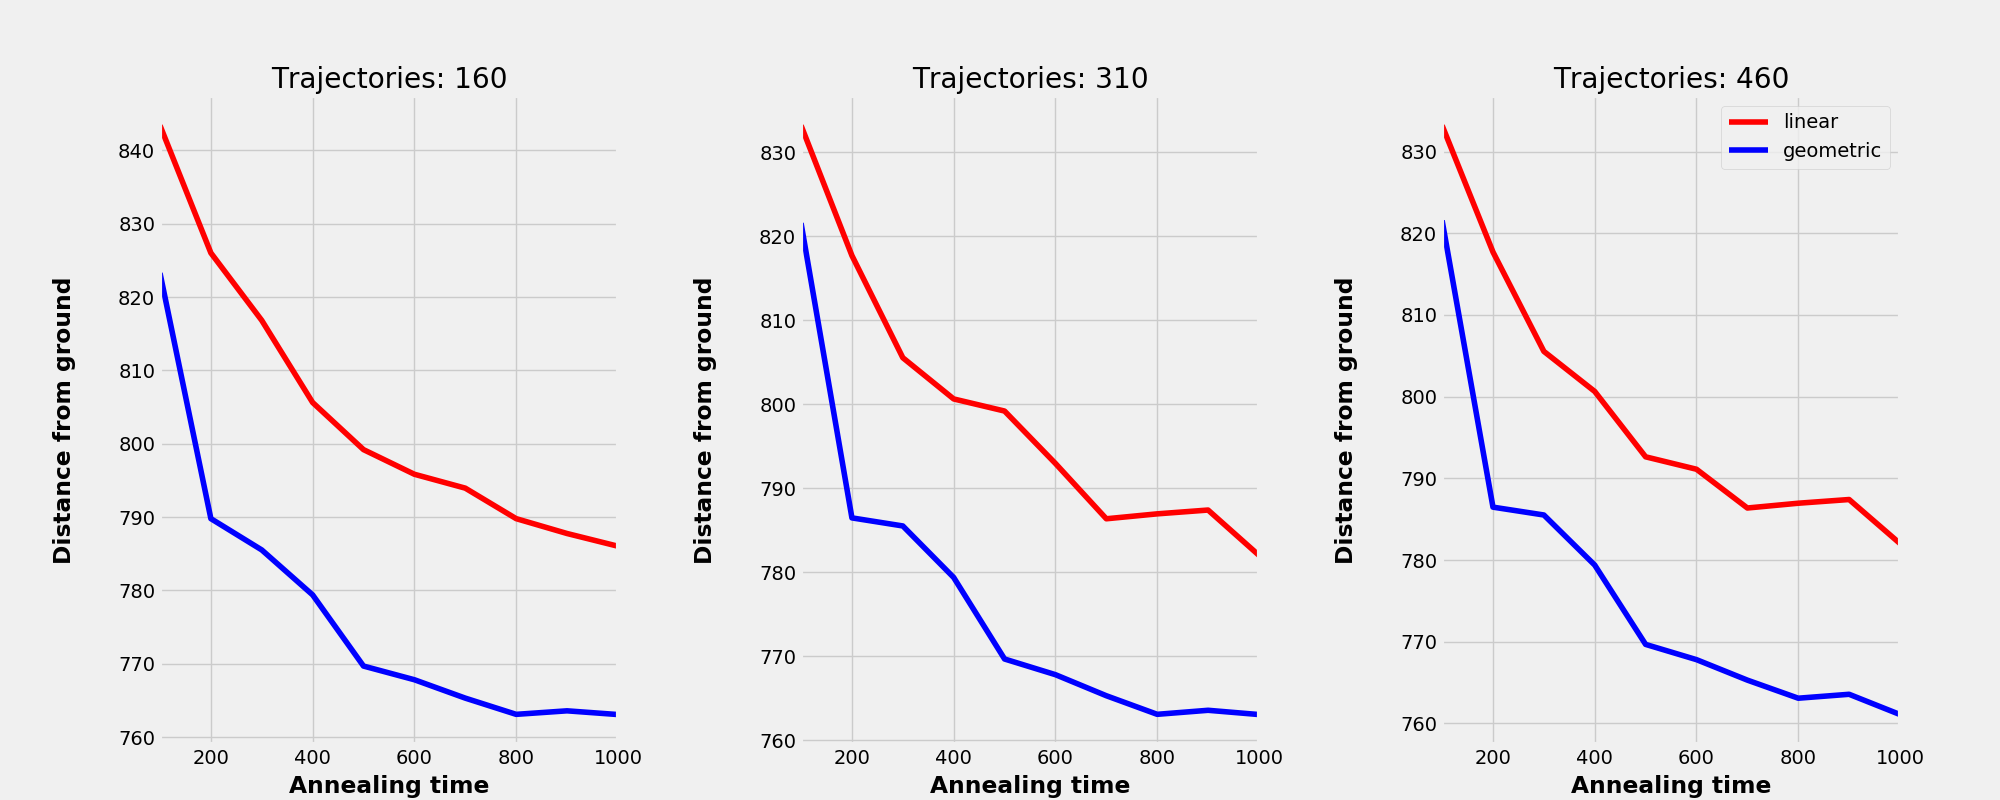
\includegraphics[width=1.0\textwidth]{HYP-24_chimera_128.pdf}
	\caption{
	Difference between the true ground state, and the solution found by oneSolver for the Chimera graph with $L=128$ vertices, and
	various repetitions. ``linear'', and ``geometric'' reefer to the possible schedules of the inverse Boltzmann temperature, $\beta$,  
	that is used in the Metropolis-Hastings update.}
	\label{fig1}
\end{figure}
%
\begin{figure}[h!]
	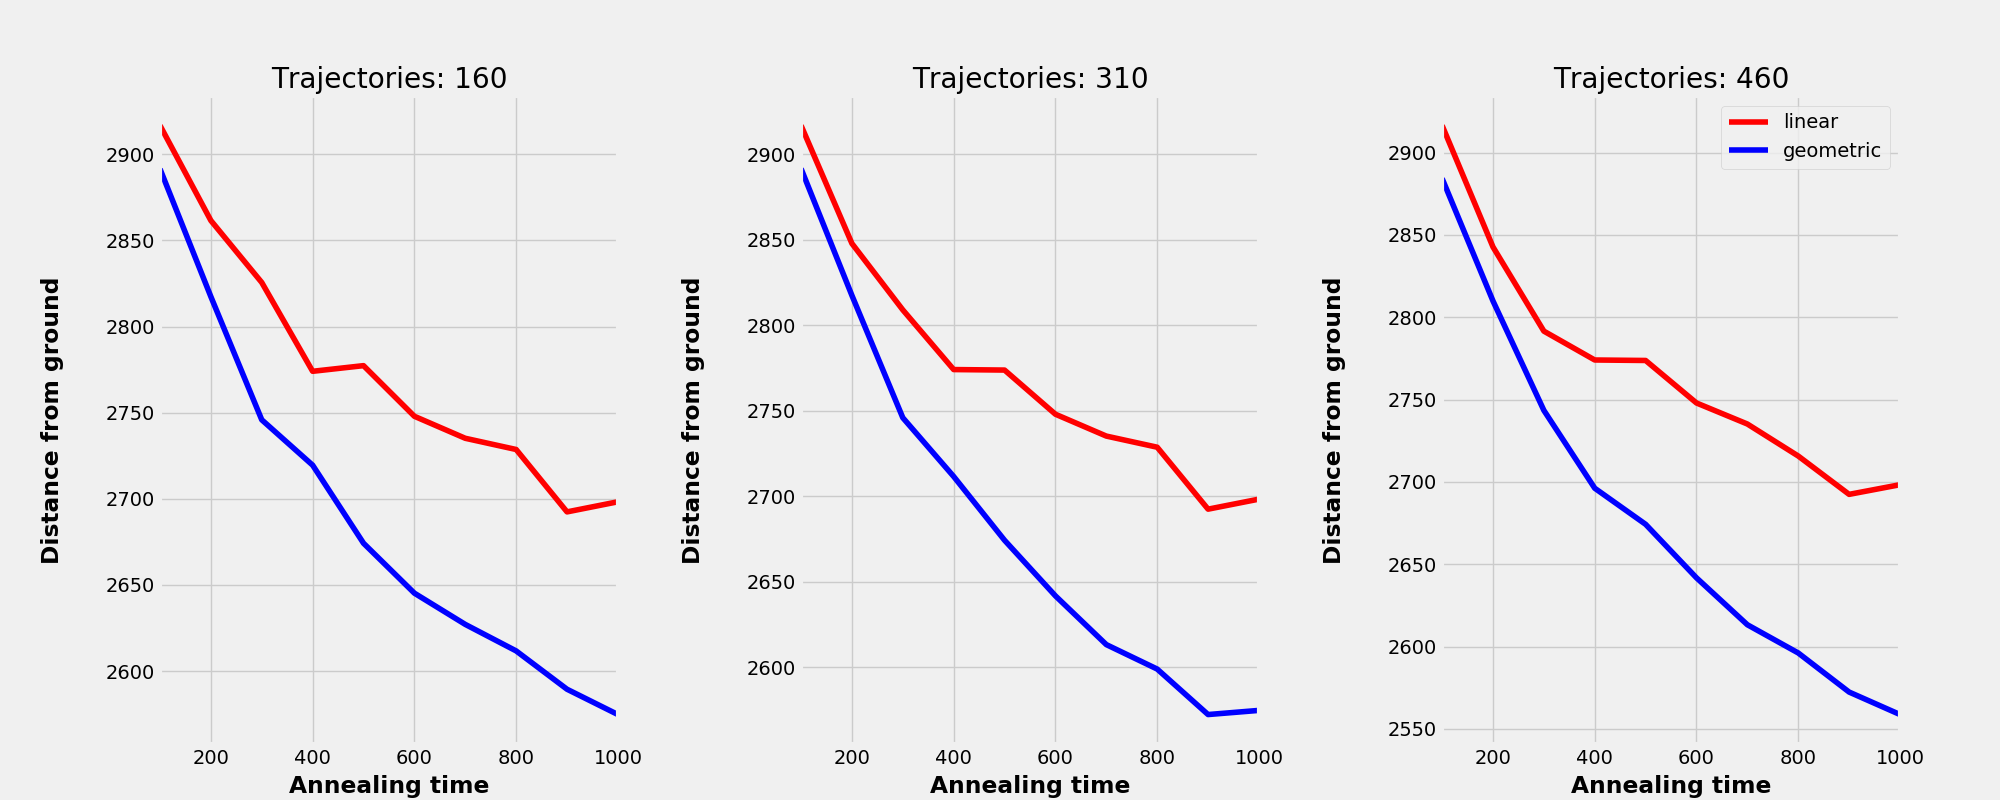
\includegraphics[width=1.0\textwidth]{HYP-24_chimera_512.pdf}
	\caption{As above, for the Chimera graph with $L=512$ vertices.}
	\label{fig2}
\end{figure}
%
\begin{figure}[h!]
	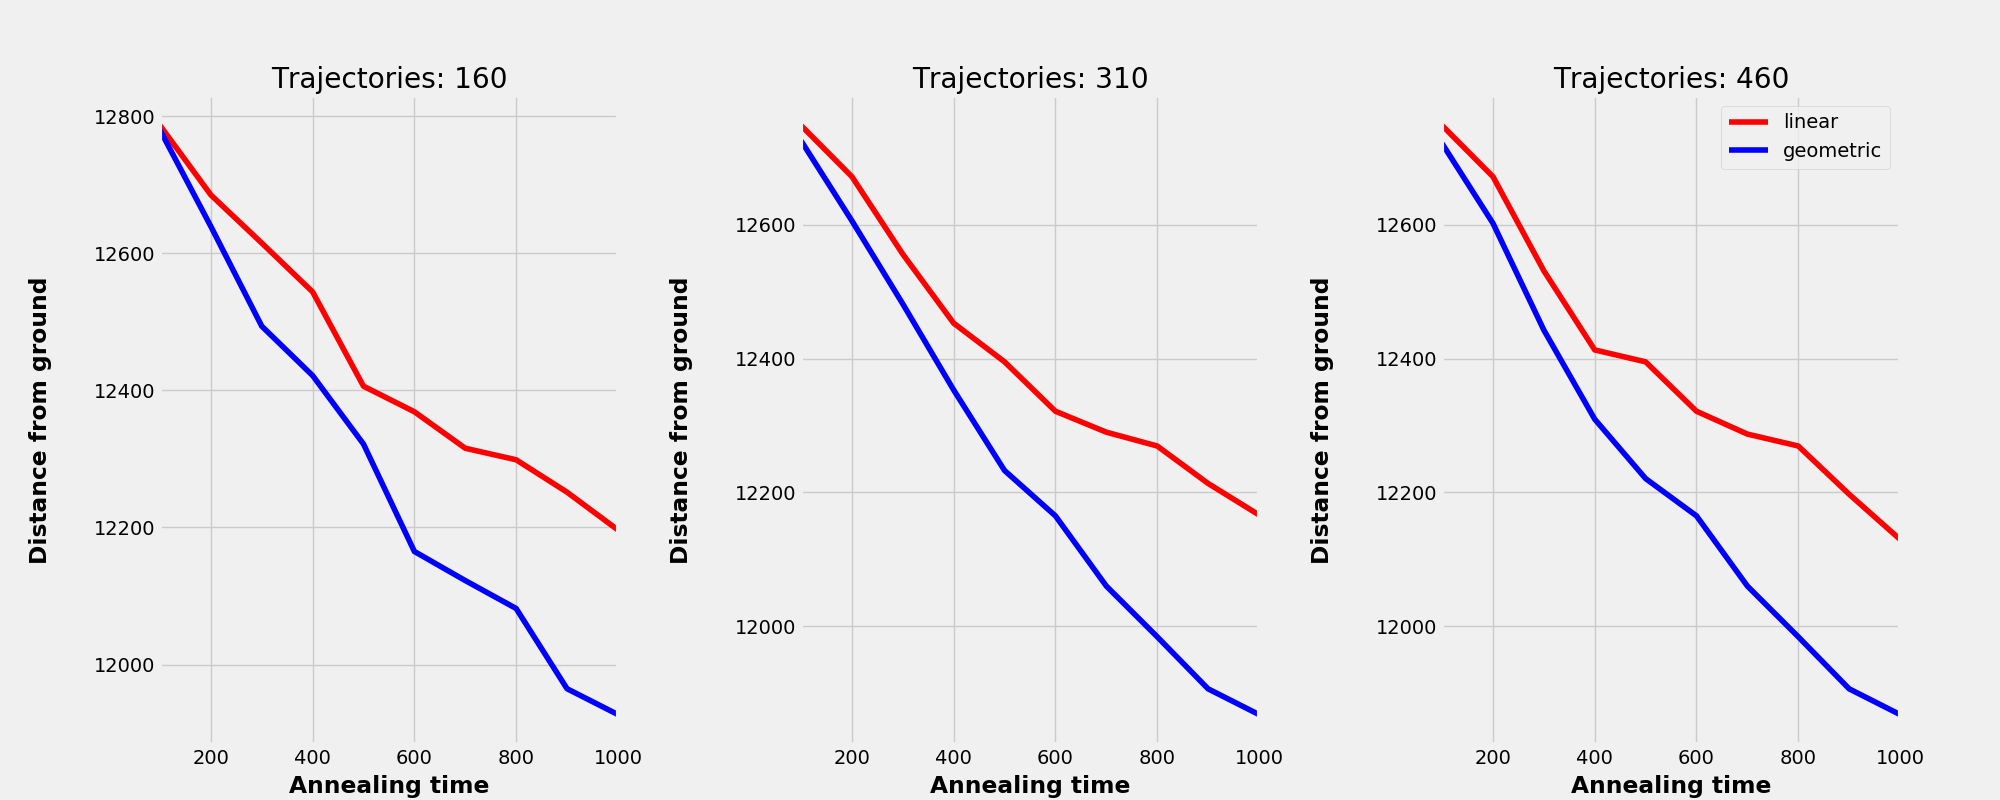
\includegraphics[width=1.0\textwidth]{HYP-24_chimera_2048.pdf} 
	\caption{As above, for the Chimera graph with $L=2014$ vertices.}
	\label{fig3}
\end{figure}

\newpage

\section{Conclusions}

For details concerning droplet instances cf.
M. M. Rams, M. Mohseni, B. Gardas,  ``\emph{Heuristic optimization and sampling with tensor networks for quasi-2D spin glass problems}'', 
\href{https://arxiv.org/abs/1811.06518}{arxiv.org/abs/1811.06518 (2018)}. Further details, including additional testing problems with known solutions, 
can also be found at \href{https://github.com/marekrams/tnac4o}{https://github.com/marekrams/tnac4o}.

As can been seen in Figs.~\ref{fig1} -~\ref{fig3}, the difference between the true ground state (obtained by the tensor network solver), and the solution found by oneSolver 
increases with the increasing system size (number of vertices). This behaviour was to be expected as the problem is NP-hard.
Moreover, the geometric inverse temperature schedule, performed better than the linear one.  Nevertheless, oneSolver was unable 
to find the correct ground state in \emph{any} of the considered cases. 

That being said, the issue is not with the implementation (which is efficient) but rather with the algorithm itself, which in a way is too simplistic to capture sophisticated interactions
between spins encoded in the droplet instances.

\section{Recommendation}

Based on the performed benchmarks, it is therefore recommended to implement solvers that incorporate more clever spin updates. 
A good starting point in this context would be the population annealing, and parallel tempering. More sophisticated approaches that 
could also be incorporated are based on tensor networks, tropical algebras, and Lagrange multipliers. 

\end{document}          
